\chapter{Anleitung zur Simulation}\label{ch:Anleitung}  
\section{Simulation mit 5-Punkte Schema}
\textbf{1. Zeichnen eines aussagekräftigen Schemas}\\ 
Die Abbildung \ref{fig:Doppelpendel} zeichnet eines aussagekräftigen Schemas des Doppelpendels. 

\textbf{2. Aufstellen der Zustandsgleichungen}\\ 
Die Zustandsvariablen sind die Winkel $\varphi_1$ und $\varphi_2$ sowie deren Ableitungen $\dot{\varphi}_1$ und $\dot{\varphi}_2$. 
\begin{align}
\mathbf{x} &= \begin{bmatrix} 
\varphi_1 \\ 
\dot{\varphi}_1 \\ 
\varphi_2 \\ 
\dot{\varphi}_2 
\end{bmatrix}, &
\frac{\mathbf{d}}{\mathbf{dt}} \mathbf{x} &= \begin{bmatrix} 
\dot{\varphi}_1 \\ 
\ddot{\varphi}_1 \\ 
\dot{\varphi}_2 \\ 
\ddot{\varphi}_2 
\end{bmatrix}
\end{align}

\textbf{3. Aufstellen der Bilanzgleichungen}\\ 
Hier werden die Bilanzgleichungen für die kinetische und potentielle Energie aufgestellt:\\
\begin{align}
E &= \frac{1}{2} \cdot m_1 \cdot \left( \dot{x}_1^2 + \dot{y}_1^2 \right) + \frac{1}{2} \cdot m_2 \cdot \left( \dot{x}_2^2 + \dot{y}_2^2 \right) + \frac{1}{2} \cdot J_1 \cdot \dot{\varphi}_1^2 + \frac{1}{2} \cdot J_2 \cdot \dot{\varphi}_2^2
\end{align}
\begin{align}
U = -m_1  \cdot g \cdot s_1 \cdot \cos\varphi_1 - m_2 \cdot g \cdot (l_1 \cdot \cos\varphi_1 + s_2 \cdot \cos\varphi_2)
\end{align}

Mit Euler-Lagrange-Gleichung wird die Lagrange-Funktion $L$ aufgestellt:
\begin{align}
L &= E - U
\end{align}

Dann werden die Ableitungen der Lagrange-Funktion $L$ nach den Zustandsvariablen $\varphi_1$, $\varphi_2$, $\dot{\varphi}_1$, $\dot{\varphi}_2$ aufgestellt:
\begin{align}
\frac{d}{dt}\left(\frac{\partial L}{\partial \dot{\varphi}_1}\right) - \frac{\partial L}{\partial \varphi_1} &= 0 \\
\frac{d}{dt}\left(\frac{\partial L}{\partial \dot{\varphi}_2}\right) - \frac{\partial L}{\partial \varphi_2} &= 0
\end{align}

Die Ableitungen der Lagrange-Funktion $L$ ergeben die Bewegungsgleichungen:
\begin{align}
a_{11} \cdot \ddot{\varphi}_1 + a_{12} \cdot \ddot{\varphi}_2 + b_1 &= 0 \\
a_{12} \cdot \ddot{\varphi}_1 + a_{22} \cdot \ddot{\varphi}_2 + b_2 &= 0
\end{align}

Die Koeffizienten $a_{11}$, $a_{12}$, $a_{22}$, $b_1$ und $b_2$ werden aus den Ableitungen der Lagrange-Funktion $L$ bestimmt:
\begin{align}
a_{11} &= \frac{J_1}{m_1 \cdot l_1^2} + \frac{m_2}{m_1} + \frac{s_1^2}{l_1^2} \\
a_{12} &= \frac{m_2 \cdot s_2}{m_1 \cdot l_1} \cdot \cos(\varphi_1 - \varphi_2) \\
a_{22} &= \frac{J_2}{m_1 \cdot l_1^2} + \frac{m_2 \cdot s_2^2}{m_1 \cdot l_1^2} \\
b_1 &= \frac{m_2 \cdot s_2}{m_1 \cdot l_1} \cdot \dot{\varphi}_2^2 \cdot \sin(\varphi_1 - \varphi_2) + \left( \frac{s_1}{l_1} + \frac{m_2}{m_1} \right) \cdot \frac{g}{l_1} \cdot \sin\varphi_1 \\
b_2 &= -\frac{m_2 \cdot s_2}{m_1 \cdot l_1} \cdot \dot{\varphi}_1^2 \cdot \sin(\varphi_1 - \varphi_2) + \frac{m_2 \cdot g \cdot s_2}{m_1 \cdot l_1^2} \cdot \sin\varphi_2
\end{align}

Danach werden die Bewegungsgleichungen umgestellt, um die Beschleunigungen $\ddot{\varphi}_1$ und $\ddot{\varphi}_2$ zu erhalten:
\begin{align}
\ddot{\varphi}_1 &= \frac{-a_{22} \cdot b_1 + a_{12} \cdot b_2}{a_{11} \cdot a_{22} - a_{12}^2} \\
\ddot{\varphi}_2 &= \frac{a_{12} \cdot b_1 - a_{11} \cdot b_2}{a_{11} \cdot a_{22} - a_{12}^2}
\end{align}

\textbf{4. Aufstellen der statischen Beziehungen}\footnote{Doppelpendel, Wikipedia. Verfügbar unter: \href{https://de.wikipedia.org/w/index.php?title=Doppelpendel&oldid=251882175}{de.wikipedia.org}}\\
Die Positionen werden wie folgt definiert:
\begin{align}
x_1 &= s_1 \cdot \sin\varphi_1 & y_1 &= s_1 \cdot \cos\varphi_1 \\
x_2 &= l_1 \cdot \sin\varphi_1 + s_2 \cdot \sin\varphi_2 & y_2 &= l_1 \cdot \cos\varphi_1 + s_2 \cdot \cos\varphi_2
\end{align}

Danach werden die Ableitungen der Positionen $x_1$, $y_1$, $x_2$ und $y_2$ nach der Zeit $t$ aufgestellt, um die Geschwindigkeiten $\dot{x}_1$, $\dot{y}_1$, $\dot{x}_2$ und $\dot{y}_2$ zu bestimmen:
\begin{align}
\dot{x}_1 &= s_1 \cdot \dot{\varphi}_1 \cdot \cos\varphi_1 & \dot{y}_1 &= -s_1 \cdot \dot{\varphi}_1 \cdot \sin\varphi_1 \\
\dot{x}_2 &= l_1 \cdot \dot{\varphi}_1 \cdot \cos\varphi_1 + s_2 \cdot \dot{\varphi}_2 \cdot \cos\varphi_2 & \dot{y}_2 &= -l_1 \cdot \dot{\varphi}_1 \cdot \sin\varphi_1 - s_2 \cdot \dot{\varphi}_2 \cdot \sin\varphi_2
\end{align}

\textbf{5. Zeichnen eines Blockschaltbildes}\\ 
Wenn vorherige Schritte erfolgreich durchgeführt wurden, kann ein Blockschaltbild gezeichnet werden. Die Abbildung \ref{fig:Blockschaltbild} zeigt das Blockschaltbild des Doppelpendels und in slx-Datei \codefile{Doppelpendel\_5\_Punkte\_Schema.slx} simuliert. Das Solver ist hier \textit{ode15s} \footnote{Choose an ODE Solver. Verfügbar unter: \href{https://de.mathworks.com/help/matlab/math/choose-an-ode-solver.html}{de.mathworks.com}} mit einer Maximale Schrittweite von $1e-4$ und einer Relativen Toleranz von $1e-8$.
\begin{figure}[H]
  \centering
  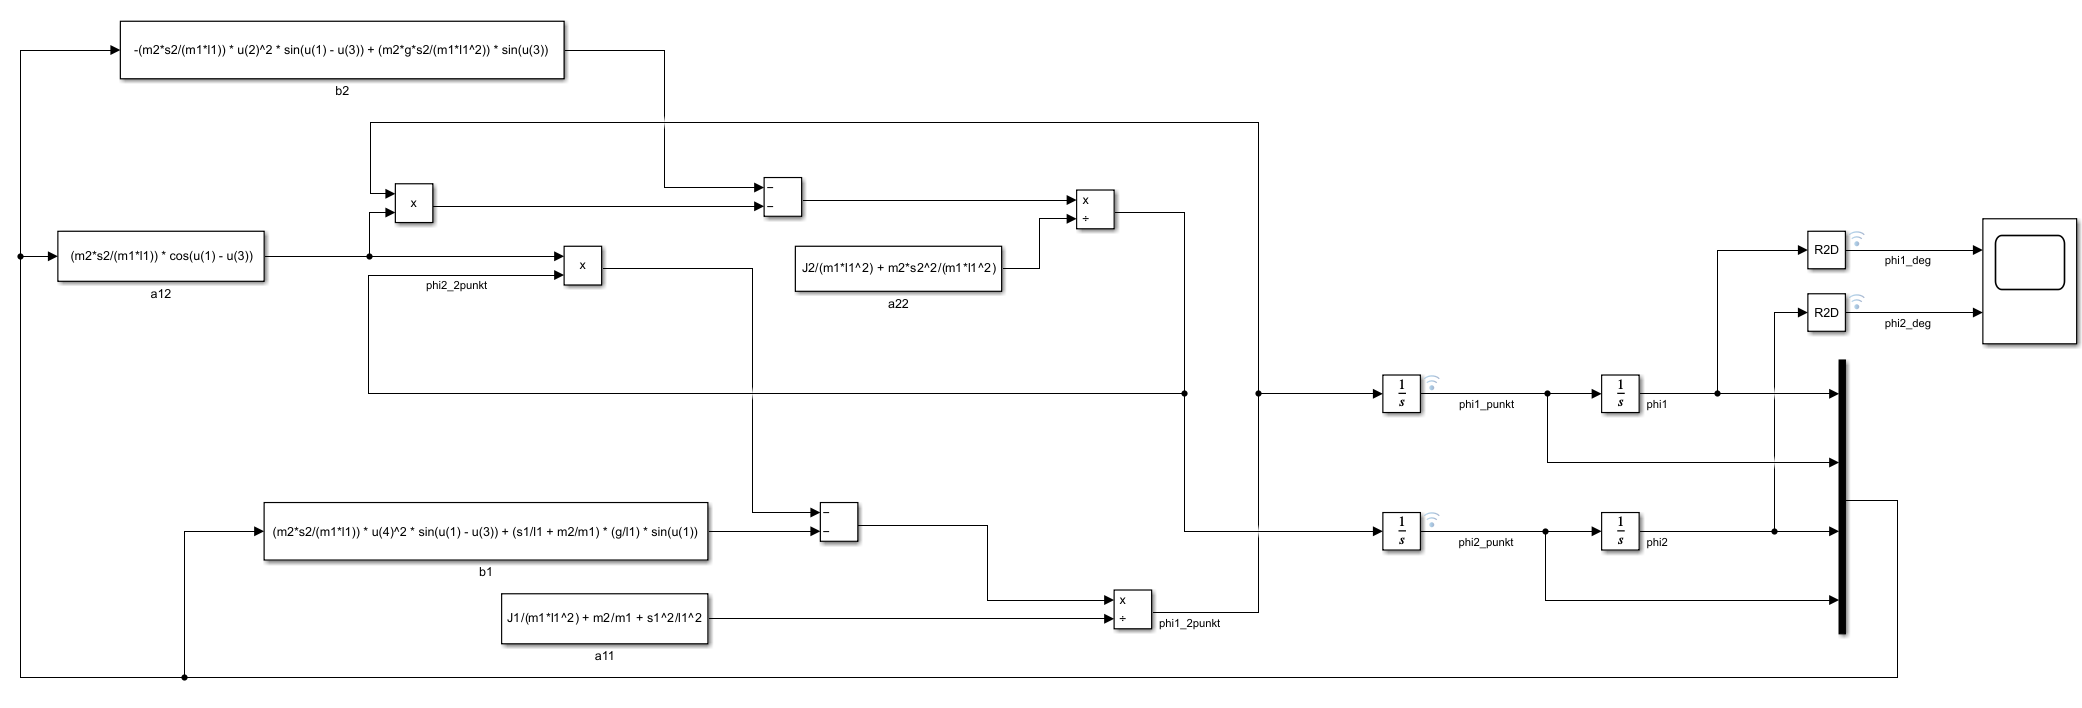
\includegraphics[width=1\textwidth]{figures/Blockschaltbild.png}
  \caption{Blockschaltbild des Doppelpendels}
  \label{fig:Blockschaltbild}
\end{figure}

\section{Simulation mit Zustandsraum}
\textbf{Linearisierung am Gleichgewichtspunkt}\\
Der Gleichgewichtspunkt ist definiert als:
\begin{align}
  \varphi_1 &= 0, &\dot{\varphi}_1 &= 0, &\varphi_2 &= 0, &\dot{\varphi}_2 &= 0
\end{align}

Zur Linearisierung werden hier die partiellen Ableitungen berechnet:
\begin{align}
  \frac{\partial b_1}{\partial \varphi_1} &= \left(\frac{s_1}{l_1} + \frac{m_2}{m_1}\right) \cdot \frac{g}{l_1} \cdot \cos(\varphi_1)\Big|_{\varphi_1=0} = \left(\frac{s_1}{l_1} + \frac{m_2}{m_1}\right) \cdot\frac{g}{l_1} \\
  \frac{\partial b_1}{\partial \varphi_2} &= 0 \\
  \frac{\partial b_1}{\partial \dot{\varphi}_1} &= 0 \\
  \frac{\partial b_1}{\partial \dot{\varphi}_2} &= 0 \\
  \frac{\partial b_2}{\partial \varphi_1} &= 0 \\
  \frac{\partial b_2}{\partial \varphi_2} &= \frac{m_2 \cdot g \cdot s_2}{m_1 \cdot l_1^2} \cdot \cos(\varphi_2)\Big|_{\varphi_2=0} = \frac{m_2 \cdot g \cdot s_2}{m_1 \cdot l_1^2} \\
  \frac{\partial b_2}{\partial \dot{\varphi}_1} &= 0 \\
  \frac{\partial b_2}{\partial \dot{\varphi}_2} &= 0
\end{align}

Aus den Ableitungen der Lagrange-Funktion $L$ ergeben sich weitere
partiellen Ableitungen, was in der folgenden Matrix $\mathbf{A}$
braucht. Das wird in m-Datei \codefile{Doppelpendel\_Linearisierung.m}
implementiert.

\textbf{Zustandsraumdarstellung}\\
Mit dem Zustandsvektor $\mathbf{x} = [\varphi_1, \dot{\varphi}_1, \varphi_2, \dot{\varphi}_2]^T$ wird das System in Zustandsraumdarstellung beschrieben:
\begin{align}
  \dot{\mathbf{x}} &= \mathbf{A}\mathbf{x} + \mathbf{B}\mathbf{u} \\
  \mathbf{y} &= \mathbf{C}\mathbf{x} + \mathbf{D}\mathbf{u}
\end{align}

Die Systemmatrix $\mathbf{A}$ wird konstruiert als:
\begin{align}
  \mathbf{A} = 
  \begin{bmatrix}
    0 & 1 & 0 & 0 \\
    \frac{\partial \ddot{\phi}_1}{\partial \phi_1} & \frac{\partial \ddot{\phi}_1}{\partial \dot{\phi}_1} & \frac{\partial \ddot{\phi}_1}{\partial \phi_2} & \frac{\partial \ddot{\phi}_1}{\partial \dot{\phi}_2} \\
    0 & 0 & 0 & 1 \\
    \frac{\partial \ddot{\phi}_2}{\partial \phi_1} & \frac{\partial \ddot{\phi}_2}{\partial \dot{\phi}_1} & \frac{\partial \ddot{\phi}_2}{\partial \phi_2} & \frac{\partial \ddot{\phi}_2}{\partial \dot{\phi}_2}
  \end{bmatrix}
\end{align}

Nachdem man m-Datei \codefile{Doppelpendel\_Linearisierung.m} durchgeführt hat, wird alle Matrizen berechnet. Schließlich wird die Blockschaltbild des Zustandsraummodells in der Abbildung \ref{fig:Blockschaltbild_Zustandsraum} gezeichnet und in slx-Datei \codefile{Doppelpendel\_Zustandsraum.slx} simuliert. Das Solver wird hier gleiche wie die Simulation mit 5-Punkte Schema eingestellt.
\begin{figure}[H]
  \centering
  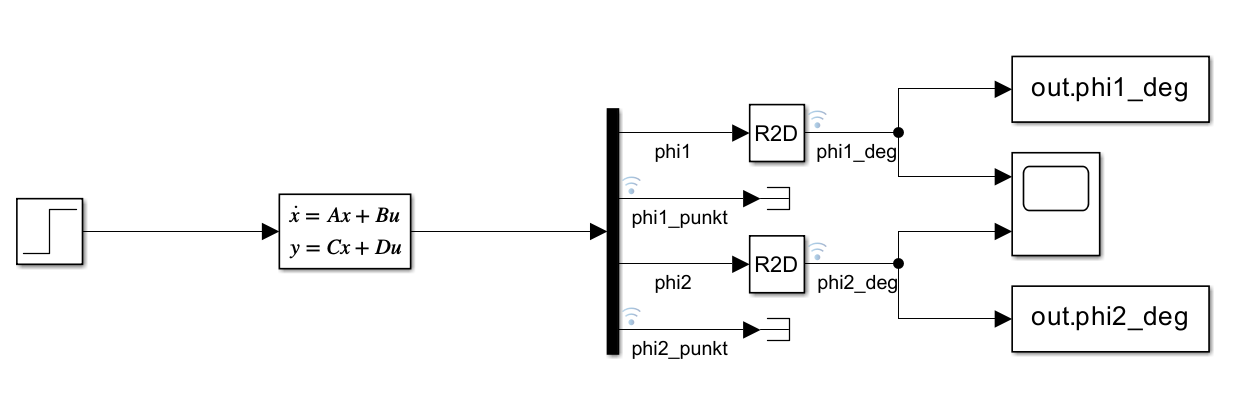
\includegraphics[width=0.7\textwidth]{figures/Blockschaltbild_Zustandsraum.png}
  \caption{Blockschaltbild des Zustandsraummodells}
  \label{fig:Blockschaltbild_Zustandsraum}
\end{figure}

\section{Simulation in Matlab (ohne Simulink)}
Das Skript erstellt von der gleichen Gleichungen, was die Simulation mit 5-Punkte Schema genutzt hat. Die Simulation wird in m-Datei \codefile{Doppelpendel.m} durchführen und die Funktion \codefile{xpunkt\_Doppelpendel.m} aufrufen, um die Differentialgleichung aufzustellen. Danach wird die Differentialgleichung mit \textit{ode15s} gelöst. Die Simulation wird mit den gleichen Parametern und Anfangsbedingungen wie die Simulation in Simulink durchführen. 

Hier werden die Simulation erweitert, um ein Dreifachpendel zu simulieren. Das kann man in der m-Datei \codefile{Dreifachpendel.m} durchführen. Die m-Datei \codefile{Dreifachpendel.m} wird die Funktion \codefile{xpunkt\_Dreifachpendel.m} aufrufen und mit ähnlichen Lösungsweisen wie die Simulation des Doppelpendels durchführen. 

